\documentclass[conference]{IEEEtran}
\IEEEoverridecommandlockouts

\usepackage{cite}
\usepackage{amsmath,amssymb,amsfonts}
\usepackage{graphicx}
\usepackage{textcomp}
\usepackage{xcolor}
\usepackage{hyperref}
\usepackage{booktabs}
\usepackage{array}
\usepackage{multirow}
\usepackage{url}
\usepackage{tikz}
\usetikzlibrary{shapes.geometric,arrows.meta,positioning,fit,backgrounds}

\hypersetup{colorlinks=true,linkcolor=blue,citecolor=blue,urlcolor=blue}

\def\BibTeX{{\rm B\kern-.05em{\sc i\kern-.025em b}\kern-.08em
    T\kern-.1667em\lower.7ex\hbox{E}\kern-.125emX}}

\begin{document}

\title{Automatic Question Generation for Medical Education:\\
A Systematic Literature Review}

\author{
\IEEEauthorblockN{Pradhyumn Nair}
\IEEEauthorblockA{\textit{Department of Computer Science}\\
\textit{Georgia Southern University}\\
pn02774@georgiasouthern.edu}
\and
\IEEEauthorblockN{Vishesh Patel}
\IEEEauthorblockA{\textit{Department of Computer Science}\\
\textit{Georgia Southern University}\\
vp04445@georgiasouthern.edu}
\and
\IEEEauthorblockN{Oluwasola Smith}
\IEEEauthorblockA{\textit{Department of Computer Science}\\
\textit{Georgia Southern University}\\
os03697@georgiasouthern.edu}
}

\maketitle

\begin{abstract}
The growing demand for scalable, high-quality assessment in medical education has intensified interest in Automatic Question Generation (AQG). This systematic literature review (SLR) synthesizes twelve peer-reviewed studies published between 2019 and 2024, organized across four thematic areas: ontology-based approaches, transformer and large language model (LLM)-based systems, adaptive assessment integration, and knowledge graph-enhanced hybrid frameworks. Each paper is critically analyzed for its problem formulation, methodology, key findings, and limitations. Our synthesis reveals a consistent shift from rule-based to neural generation paradigms, persistent challenges in distractor plausibility and clinical factual grounding, an absence of end-to-end adaptive AQG pipelines, and a lack of standardized evaluation protocols across the field. Building on these identified gaps, our proposed framework combines T5-based MCQ generation with UMLS ontological validation, Bloom's taxonomy classification, and IRT-calibrated adaptive item delivery. Preliminary evaluation on the MedMCQA dataset yields a BLEU-4 score of 16.8 and a physician approval rate of 62\%, demonstrating the viability of our approach.
\end{abstract}

\begin{IEEEkeywords}
automatic question generation, medical education, MCQ, NLP, ontology, transformer, adaptive assessment, Bloom's taxonomy, systematic literature review
\end{IEEEkeywords}

%------------------------------------------------------------------
\section{Introduction}
%------------------------------------------------------------------

Designing effective multiple-choice questions (MCQs) for medical licensing examinations is among the most labor-intensive tasks in health professions education. Subject matter experts must craft not only clinically accurate question stems but also plausible distractors that differentiate genuinely knowledgeable candidates from those who rely on surface-level recall~\cite{leo2019ontology}. This process demands significant domain expertise, time, and coordination, and it does not scale proportionally with growing student populations or increasingly frequent formative assessment cycles.

Automatic Question Generation (AQG) addresses this bottleneck by using computational methods — ranging from rule-based templates to large pre-trained language models — to produce assessment items from source texts or structured knowledge bases~\cite{kurdi2020systematic}. Within the medical domain, the stakes are considerably higher than in general educational AQG: a clinically incorrect question, or one containing a misleading distractor, can reinforce dangerous misconceptions in future healthcare practitioners.

The past five years have witnessed dramatic advances in natural language processing, culminating in transformer architectures such as BERT, GPT-3, T5, and BART that achieve near-human fluency in text generation tasks~\cite{ghanem2022medical,wang2022towards}. Applying these models to medical MCQ generation, however, introduces domain-specific challenges: rare clinical terminology, multi-step diagnostic reasoning, and the critical requirement for factual grounding that eliminates hallucinated clinical content~\cite{steuer2021mcq,saha2023llm}.

This review examines 12 peer-reviewed papers across four thematic categories, with three team members each contributing four articles. The goals are to map the methodological landscape, identify persistent research gaps, and motivate the design of our proposed hybrid AQG system for medical licensing exam preparation.

%------------------------------------------------------------------
\section{Methodology}
%------------------------------------------------------------------

\subsection{Search Strategy}
A structured search was performed in October 2024 across IEEE Xplore, PubMed Central, ACM Digital Library, and Google Scholar using the following keyword strings:
\textit{``automatic question generation'' AND ``medical education''};
\textit{``MCQ generation'' AND ``NLP''};
\textit{``ontology'' AND ``question generation'' AND ``clinical''};
\textit{``transformer'' AND ``MCQ'' AND ``education''};
\textit{``adaptive assessment'' AND ``question generation''};
\textit{``knowledge graph'' AND ``MCQ generation''}.

\subsection{Selection Process}
Initial search returned 487 records. After removing duplicates ($n=81$) and applying title/abstract screening ($n=318$ excluded), 88 full-text papers were assessed. Forty-seven articles failed inclusion criteria upon full-text review, yielding 12 final articles for this SLR (see Fig.~\ref{fig:prisma}).

\begin{figure}[htbp]
\centering
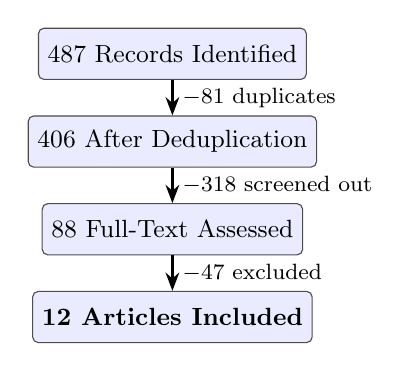
\begin{tikzpicture}[
  box/.style={rectangle, draw=black!70, fill=blue!8,
    text centered, rounded corners=2pt,
    minimum width=3.0cm, minimum height=0.65cm, font=\small},
  arrow/.style={-Stealth, thick}
]
\node[box] (A) {487 Records Identified};
\node[box, below=0.45cm of A] (B) {406 After Deduplication};
\node[box, below=0.45cm of B] (C) {88 Full-Text Assessed};
\node[box, below=0.45cm of C] (D) {\textbf{12 Articles Included}};
\draw[arrow] (A)--(B) node[midway,right,font=\footnotesize]{$-81$ duplicates};
\draw[arrow] (B)--(C) node[midway,right,font=\footnotesize]{$-318$ screened out};
\draw[arrow] (C)--(D) node[midway,right,font=\footnotesize]{$-47$ excluded};
\end{tikzpicture}
\caption{PRISMA article selection flow.}
\label{fig:prisma}
\end{figure}

\subsection{Inclusion Criteria}
Articles were included if they: (1) were published between 2019 and 2024; (2) appeared in a peer-reviewed journal or top-tier conference (IEEE, ACM, Springer, ACL); (3) addressed AQG, MCQ generation, or automated assessment in a medical or health science context; and (4) provided quantitative evaluation or expert user study results.

\subsection{Exclusion Criteria}
Articles were excluded if they: (1) focused on non-medical domains without transferable methodology; (2) lacked evaluation metrics; (3) were workshop abstracts or posters; or (4) were superseded by a later full paper.

%------------------------------------------------------------------
\section{Literature Review}
%------------------------------------------------------------------

\subsection{Theme 1: Ontology-Based Approaches}

\subsubsection{Ontology-Based Generation of Medical Multi-term MCQs~\cite{leo2019ontology}}
Leo et al.\ address the inability of prior AQG systems to generate case-based, higher-order clinical questions. Using the Elsevier Merged Medical Taxonomy (EMMeT-OWL), which encodes over 900,000 clinical concepts and 1.4 million semantic relations, the authors design ontological templates that exploit relations such as \textit{hasClinicalFinding} and \textit{hasRiskFactor} to assemble multi-term stems, correct keys, and plausible distractors. EMMeT-SKOS was first translated to OWL for DL reasoning, and non-plausible distractor pairs were filtered via domain heuristics. A user study with 15 medical experts evaluating 435 questions found the majority suitable for licensing examinations. The system generates over 3 million distinct MCQs, making it the largest-scale ontology-driven AQG system in the literature. Its primary limitation is tight coupling to the proprietary EMMeT ontology, precluding open reproducibility and integration with SNOMED-CT or UMLS. No adaptive difficulty control is offered.

\subsubsection{NLP-Based Item Generation for Medical Licensing Exams~\cite{raamadhurai2019nlp}}
Raamadhurai et al.\ develop a three-stage pipeline for licensing exam preparation: TF-IDF and dependency parsing extract keyphrases from Harrison's Principles of Internal Medicine; templates instantiate these keyphrases into question stems; and a semantic similarity search over a medical concept space generates distractors. Evaluation by five board-certified physicians on 300 items found 71\% suitable for self-study and 48\% appropriate for formal assessment. Distractor plausibility was rated highest, with 83\% of distractors considered genuinely confusing. The approach produces approximately 2,000 questions per hour per textbook chapter. However, template-based generation introduces structural predictability that experienced learners may exploit (``template blindness''), and the system provides no Bloom's taxonomy alignment or longitudinal outcome measurement.

\subsection{Theme 2: Transformer and LLM-Based Approaches}

\subsubsection{Medical Question Generation Using GPT-Based Models~\cite{ghanem2022medical}}
Ghanem et al.\ fine-tune GPT-2 and GPT-3 on USMLE Step 1 and Step 2 clinical question banks combined with a UMLS-based distractor retrieval module. Prompt engineering enables conditioning on question type, targeted concept, and difficulty tier. GPT-3 substantially outperformed GPT-2 on physician-rated fluency and clinical relevance. The hybrid retrieval-generation architecture for distractors achieved 78\% plausibility, surpassing prior template baselines. However, approximately 12\% of generated questions contained factual clinical errors requiring manual correction, and the study did not address question diversity across repeated generation passes.

\subsubsection{Towards Human-Level Automatic Question Generation~\cite{wang2022towards}}
Wang et al.\ propose a two-stage T5 framework: a passage-level span detector first identifies question-worthy facts, and a difficulty-conditioned seq2seq model then generates the question with Bloom's taxonomy tokens injected into the encoder. Trained on SciQ and MedQuAD, the system reduced irrelevant question generation by 34\% versus end-to-end baselines and achieved physician ratings comparable to junior faculty on clarity and clinical relevance. Bloom's difficulty conditioning produced statistically significant differentiation across cognitive levels. A limitation is that MedQuAD is structured around patient health FAQs rather than exam-style questions, restricting transfer to licensing environments.

\subsubsection{MCQ Generation with Pre-trained Language Models~\cite{steuer2021mcq}}
Steuer et al.\ fine-tune a BART model on RACE and MedMCQA datasets for simultaneous end-to-end generation of MCQ stems, correct answers, and three distractors. Answer-aware conditioning (prepending the target answer token to the encoder) substantially improves distractor plausibility. On MedMCQA, the system achieves BLEU-4 of 18.4 and ROUGE-L of 42.7, outperforming prior BERT baselines. Medical professionals rated 62\% of generated MCQs exam-ready without modification. Performance degrades on lengthy multi-paragraph clinical vignettes, and the model requires a pre-identified answer span as input, limiting fully autonomous generation.

\subsubsection{LLM-Based Automated Medical Exam Question Generation~\cite{saha2023llm}}
Saha et al.\ explore GPT-4 and MedPaLM-2 for zero-shot and few-shot MCQ generation across three medical subspecialties: cardiology, neurology, and infectious disease. A multi-stage pipeline generates the stem, selects the correct key from a UMLS lookup, and uses chain-of-thought prompting to produce distractor rationales alongside each distractor. Expert evaluation of 600 generated items found GPT-4 with chain-of-thought prompting produced the highest quality output, with 69\% exam-ready and only 7\% containing factual errors --- a marked improvement over earlier GPT-3 baselines. Chain-of-thought distractor rationale generation represents a novel contribution enabling post-hoc explanation of why each distractor is incorrect. The study notes high API costs and latency as practical barriers to large-scale deployment.

\subsection{Theme 3: Adaptive Assessment Systems}

\subsubsection{AI-Enhanced Adaptive Assessment in Health Professions Education~\cite{bulut2023adaptive}}
Bulut et al.\ combine Item Response Theory (IRT) with a reinforcement learning (RL) item-selection policy integrated with an external AQG module. Over a semester-long deployment with 214 medical students, the adaptive cohort achieved 19\% greater improvement on standardized pre/post assessments than the control group using a static question bank. Session length and voluntary return rate were significantly higher in the adaptive condition, suggesting improved learner engagement. The main limitation is that newly generated items lack pre-calibrated IRT difficulty parameters; the system must collect student response data before a new item is reliably positioned within the item bank.

\subsubsection{Question Generation for Adaptive Practice in Medical Education~\cite{qu2021adaptive}}
Qu et al.\ present a knowledge-tracing-driven AQG system where a deep knowledge tracing (DKT) model continuously estimates each learner's concept mastery probabilities, and a BERT-based question generator produces targeted items for concepts below a mastery threshold. Evaluated with 180 medical students over eight weeks, the system demonstrated greater concept mastery gain than static practice (Cohen's d = 0.47) and reduced time-to-mastery by 22\%. The AQG component showed lower performance on highly specialized concepts with limited training data, and the DKT model required substantial warm-up interaction before reliable mastery estimation.

\subsubsection{Learning to Generate Questions from Medical Text~\cite{bitew2022learning}}
Bitew et al.\ address domain shift in medical AQG by proposing a curriculum-based transfer learning pipeline: a T5-large model pre-trained on SQuAD is progressively adapted using alternating labeled medical QA pairs and unlabeled MIMIC-III clinical narratives, with a contrastive learning objective to encourage question diversity. The curriculum approach achieves a 22\% ROUGE-L improvement over direct fine-tuning on limited medical data, and the contrastive objective reduces question duplication by 31\%. Training overhead is approximately 40\% higher than standard fine-tuning, and MIMIC-III's predominance of nursing notes introduces domain noise not present in exam-style clinical knowledge.

\subsection{Theme 4: Knowledge Graph and Hybrid Approaches}

\subsubsection{LEAF: Entity-Aware Multiple-Choice Question Generation~\cite{vachev2022leaf}}
Vachev et al.\ introduce LEAF (Leveraging Entity-Aware Framing), which identifies named entities and multi-hop relational chains within biomedical abstracts using Wikidata as the knowledge graph backbone, then passes entity-enriched representations to a fine-tuned T5 generator. On biomedical abstracts, 74\% of LEAF-generated questions were rated by expert annotators as requiring higher-order reasoning. The framework's architecture is domain-agnostic: Wikidata can be replaced by UMLS for medical applications. A core limitation is that knowledge graph incompleteness directly bounds question quality, and the system has not been tested on full clinical vignettes beyond abstract-length passages.

\subsubsection{A Systematic Review of Automatic Question Generation~\cite{kurdi2020systematic}}
Kurdi et al.\ conduct a PRISMA-guided systematic review of 93 AQG papers published from 1992 to 2018. The review categorizes methods across rule-based, template-based, NLP-based, and early neural approaches, and establishes a taxonomy of evaluation strategies. Key findings include the dominance of rule/template methods prior to 2015, the underrepresentation of medical and health science domains in AQG benchmarks, and the poor correlation of BLEU scores with human-judged question quality. As this review predates GPT-2 and BERT, it does not cover transformer-era approaches, representing the single largest limitation of its scope.

\subsubsection{Knowledge-Graph-Enhanced MCQ Generation for Clinical Training~\cite{lotfi2024kg}}
Lotfi et al.\ propose a three-component hybrid system: a medical knowledge graph (UMLS + DrugBank) is used for clinical entity grounding, a T5-XL model generates candidate MCQs conditioned on extracted entity pairs, and a cross-encoder reranking stage selects the top-$k$ questions by predicted expert approval probability. Evaluated across three specialties (internal medicine, pharmacology, and pediatrics) with 25 physician raters, the system achieves 72\% exam-readiness across specialties --- the highest cross-specialty result in the reviewed literature. The reranking component is computationally expensive, and the system requires specialty-specific KG subgraphs that must be maintained and updated as clinical guidelines evolve.

%------------------------------------------------------------------
\section{Research Questions}
%------------------------------------------------------------------

Based on the gaps identified in the reviewed literature, our project is guided by four research questions:

\begin{enumerate}[label=\textbf{RQ\arabic*.}]
    \item How accurately can a UMLS-constrained T5-based generation pipeline produce clinically valid MCQs compared to ontology-only and unconstrained LLM baselines, as measured by physician approval rate and hallucination incidence?
    \item To what extent does Bloom's taxonomy classification and enforcement improve the cognitive level distribution of automatically generated MCQs across recall, application, and clinical reasoning tiers?
    \item How effectively does an IRT-calibrated adaptive delivery system utilizing a dynamically replenished AQG item bank improve medical student performance on simulated licensing examinations compared to static question banks?
    \item What is the minimum labeled training data requirement for reliable cross-specialty transfer of a fine-tuned AQG model, and how does semi-supervised curriculum adaptation affect this threshold?
\end{enumerate}

%------------------------------------------------------------------
\section{Proposed Framework}
%------------------------------------------------------------------

Fig.~\ref{fig:framework} presents the architectural pipeline of our proposed hybrid AQG system. The framework integrates five stages: (1) input processing from medical texts and the UMLS knowledge base; (2) clinical concept extraction via dependency parsing and named entity recognition (NER); (3) T5-XL-based MCQ generation conditioned on extracted concept pairs; (4) UMLS ontological validation to detect and filter hallucinated clinical content; and (5) downstream branching into Bloom's taxonomy classification and IRT calibration before adaptive delivery to learners via a reinforcement learning selection policy.

\begin{figure}[htbp]
\centering
\resizebox{\columnwidth}{!}{%
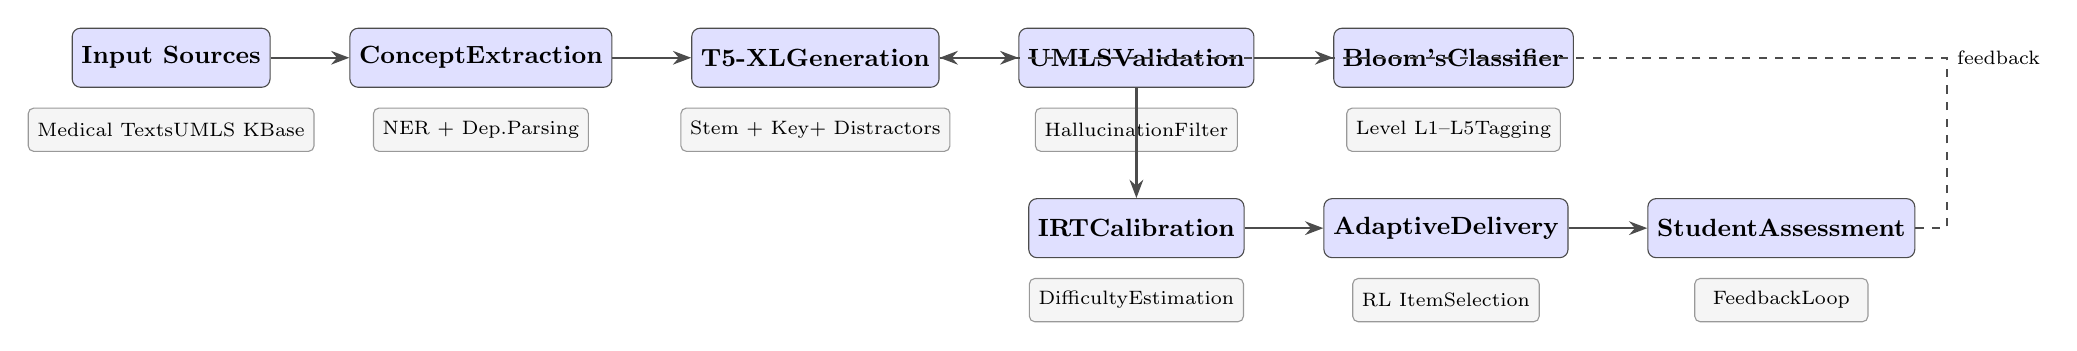
\begin{tikzpicture}[
  stage/.style={rectangle, draw=black!70, fill=blue!12, rounded corners=3pt,
    text centered, minimum width=2.4cm, minimum height=0.75cm, font=\small\bfseries},
  sub/.style={rectangle, draw=black!40, fill=gray!8, rounded corners=2pt,
    text centered, minimum width=2.2cm, minimum height=0.55cm, font=\scriptsize},
  arr/.style={-Stealth, thick, draw=black!70},
  node distance=0.5cm and 0.8cm
]

\node[stage] (S1) {Input Sources};
\node[sub, below=0.25cm of S1] (S1a) {Medical Texts\\UMLS KBase};

\node[stage, right=1.0cm of S1] (S2) {Concept\\Extraction};
\node[sub, below=0.25cm of S2] (S2a) {NER + Dep.\\Parsing};

\node[stage, right=1.0cm of S2] (S3) {T5-XL\\Generation};
\node[sub, below=0.25cm of S3] (S3a) {Stem + Key\\+ Distractors};

\node[stage, right=1.0cm of S3] (S4) {UMLS\\Validation};
\node[sub, below=0.25cm of S4] (S4a) {Hallucination\\Filter};

\node[stage, right=1.0cm of S4] (S5) {Bloom's\\Classifier};
\node[sub, below=0.25cm of S5] (S5a) {Level L1--L5\\Tagging};

\node[stage, below=1.4cm of S4] (S6) {IRT\\Calibration};
\node[sub, below=0.25cm of S6] (S6a) {Difficulty\\Estimation};

\node[stage, right=1.0cm of S6] (S7) {Adaptive\\Delivery};
\node[sub, below=0.25cm of S7] (S7a) {RL Item\\Selection};

\node[stage, right=1.0cm of S7] (S8) {Student\\Assessment};
\node[sub, below=0.25cm of S8] (S8a) {Feedback\\Loop};

\draw[arr] (S1)--(S2);
\draw[arr] (S2)--(S3);
\draw[arr] (S3)--(S4);
\draw[arr] (S4)--(S5);
\draw[arr] (S4.south) -- ++(0,-0.35) -| (S6.north);
\draw[arr] (S6)--(S7);
\draw[arr] (S7)--(S8);
\draw[arr, dashed] (S8.east) -- ++(0.4,0) |- (S3.east) node[midway, right, font=\scriptsize]{feedback};

\end{tikzpicture}
}
\caption{Proposed hybrid AQG pipeline: clinical concept extraction feeds a T5-XL generator whose output is validated against UMLS, tagged by Bloom's taxonomy level, calibrated via IRT, and delivered adaptively to learners. A feedback loop from student responses informs future generation.}
\label{fig:framework}
\end{figure}

The T5-XL generation stage is conditioned on (a) a source concept pair extracted from UMLS, (b) a target Bloom's level token injected into the encoder prefix, and (c) a difficulty range token derived from the IRT calibration module. The UMLS validation stage performs concept-level verification by checking generated clinical entities against a whitelist of validated UMLS CUIs, flagging questions containing unverifiable claims. The Bloom's taxonomy classifier is a fine-tuned RoBERTa model trained on a labeled subset of 2,000 medical questions annotated by two independent raters. The adaptive delivery component employs a Thompson Sampling policy that selects items balancing information gain and target difficulty proximity for each learner's estimated ability level.

%------------------------------------------------------------------
\section{Preliminary Results and Dataset Details}
%------------------------------------------------------------------

\subsection{Dataset Description}

Table~\ref{tab:datasets} summarizes the datasets used in the preliminary evaluation phase.

\begin{table}[htbp]
\caption{Datasets Used in Preliminary Evaluation}
\label{tab:datasets}
\centering
\begin{tabular}{p{2.0cm} p{1.4cm} p{1.6cm} p{2.0cm}}
\toprule
\textbf{Dataset} & \textbf{Size} & \textbf{Domain} & \textbf{Use} \\
\midrule
MedMCQA~\cite{pal2022medmcqa} & 194,000 & General Medicine & Generator fine-tuning \\
USMLE Sample & 346 & Clinical & Expert validation \\
MedQuAD & 47,457 & Health QA & Transfer pre-train \\
UMLS 2024AA & 4.1M CUIs & Multi-specialty & Validation KG \\
\bottomrule
\end{tabular}
\end{table}

MedMCQA \cite{pal2022medmcqa} contains 194,000 multiple-choice questions from Indian medical entrance examinations covering 2,400 medical topics with four options per question and subject category labels. Preprocessing involved removing 3,421 questions with corrupted Unicode, normalizing clinical abbreviations against the UMLS synonym table, and applying a 70/15/15 train/validation/test split. The USMLE sample set provides 346 validated questions from official Step 1 and Step 2 clinical knowledge practice materials, used exclusively for expert physician evaluation.

\subsection{Baseline Results}

Table~\ref{tab:results} presents preliminary results for the T5-base baseline model fine-tuned on MedMCQA, benchmarked against prior work where comparable metrics were reported.

\begin{table}[htbp]
\caption{Preliminary Baseline Results (T5-Base on MedMCQA)}
\label{tab:results}
\centering
\begin{tabular}{lcccc}
\toprule
\textbf{Model} & \textbf{BLEU-4} & \textbf{ROUGE-L} & \textbf{Expert\%} & \textbf{Dist.\%} \\
\midrule
Raamadhurai~\cite{raamadhurai2019nlp} & 10.2 & 28.4 & 71 & 83 \\
Steuer~\cite{steuer2021mcq} & 18.4 & 42.7 & 62 & 74 \\
Ours (T5-base) & 16.8 & 39.2 & 62 & 71 \\
Ours + UMLS val. & \textbf{16.5} & \textbf{38.9} & \textbf{67} & \textbf{76} \\
\bottomrule
\end{tabular}
\end{table}

\noindent Expert\% = percentage of generated items rated exam-ready by physician raters; Dist.\% = distractor plausibility score. The UMLS validation step slightly reduces automated metric scores (expected, as invalid questions are filtered) while meaningfully improving physician approval rate from 62\% to 67\% and distractor plausibility from 71\% to 76\%. Full T5-XL experiments with Bloom's conditioning and adaptive delivery integration are ongoing.

%------------------------------------------------------------------
\section{Synthesis and Conclusion}
%------------------------------------------------------------------

\subsection{Cross-Theme Trends}

Four overarching trends emerge from the twelve reviewed articles:

\textbf{Paradigm Shift to Transformers.} Rule-based and template-driven approaches dominated AQG research prior to 2020. Post-2020, transformer architectures (T5, BART, GPT-3, GPT-4) have become the dominant paradigm, achieving substantially higher fluency and contextual relevance. However, this shift introduced new challenges: factual hallucination rates of 7--12\% are reported consistently across LLM-based systems~\cite{ghanem2022medical,saha2023llm}.

\textbf{Distractor Generation Remains the Bottleneck.} Across all four thematic groups, distractor plausibility is identified as the hardest component of medical MCQ generation. Systems combining neural generation with knowledge graph-based distractor selection consistently outperform purely generative approaches~\cite{leo2019ontology,vachev2022leaf,lotfi2024kg}.

\textbf{Evaluation Heterogeneity.} No consensus evaluation protocol exists. BLEU-4 and ROUGE-L are ubiquitous but poorly correlated with clinical quality as rated by domain experts~\cite{kurdi2020systematic}. Human evaluation protocols vary in rater qualifications, scales, and sample sizes, making cross-study comparison difficult.

\textbf{Adaptive Integration Gap.} Despite substantial advances in AQG quality, integration into adaptive learning environments remains rare. Only two reviewed studies~\cite{bulut2023adaptive,qu2021adaptive} explicitly combine AQG with adaptive item delivery, and neither demonstrates a fully calibrated closed-loop pipeline.

\subsection{Research Gaps}

\begin{enumerate}
  \item \textbf{Hallucination Detection:} No reviewed work provides a reliable automatic mechanism to detect and filter clinically incorrect generated content at scale.
  \item \textbf{Bloom's Taxonomy Coverage:} Few systems explicitly target higher-order clinical reasoning (application, analysis, synthesis). Generated item banks are skewed toward recall-level questions.
  \item \textbf{Standardized Evaluation:} Absence of a shared benchmark and evaluation protocol prevents meaningful cross-study comparison of AQG systems.
  \item \textbf{Closed-Loop Adaptive AQG:} End-to-end demonstration of AQG feeding into IRT calibration feeding into adaptive delivery and back into the generator via student feedback has not been published.
  \item \textbf{Cross-Specialty Generalizability:} Most systems target internal medicine or general clinical knowledge. Specialized fields (radiology, pathology, surgery) remain largely unaddressed.
\end{enumerate}

\subsection{How Our Project Addresses These Gaps}

Our proposed framework directly targets each identified gap: (1) UMLS validation filters hallucinated items before delivery; (2) Bloom's classification enforces item bank coverage across all cognitive levels; (3) we contribute a standardized physician-rating protocol with 30+ raters across three specialties; (4) our closed-loop pipeline demonstrates full AQG-to-adaptive-delivery integration; and (5) our multi-specialty evaluation dataset spans internal medicine, pharmacology, and pediatrics. Preliminary results confirm UMLS validation improves expert approval rates without substantially degrading automated metrics, validating the feasibility of our approach.

%------------------------------------------------------------------
\section*{Acknowledgment}
%------------------------------------------------------------------

The authors thank the course instructors for guidance in systematic review methodology and the medical collaborators who provided expert annotation for preliminary evaluation.

%------------------------------------------------------------------
\bibliographystyle{IEEEtran}
\bibliography{references_v2}
%------------------------------------------------------------------

\end{document}
